\section{Diameter\-Circle Class Reference}
\label{classDiameterCircle}\index{DiameterCircle@{DiameterCircle}}
{\tt \#include $<$diametercircle.h$>$}

Inheritance diagram for Diameter\-Circle::\begin{figure}[H]
\begin{center}
\leavevmode
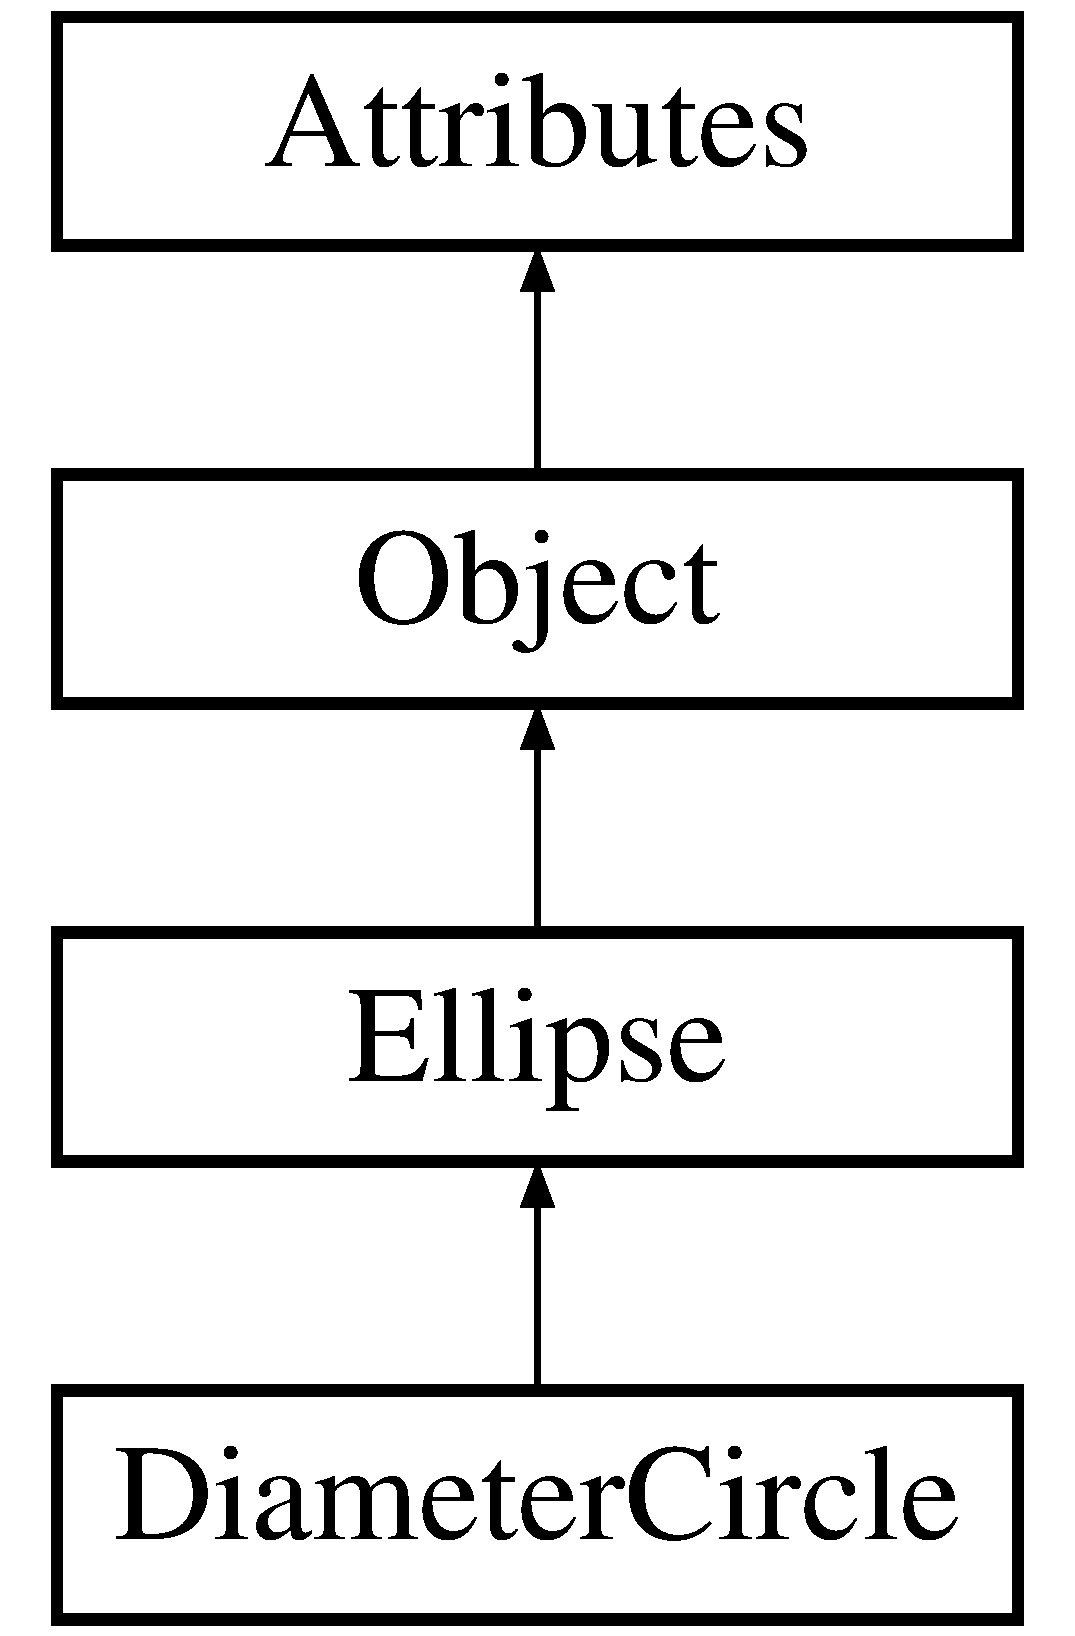
\includegraphics[height=4cm]{classDiameterCircle}
\end{center}
\end{figure}
\subsection*{Public Methods}
\begin{CompactItemize}
\item 
{\bf Diameter\-Circle} ()
\item 
{\bf Diameter\-Circle} ({\bf Coordinate} $\ast$, {\bf Coordinate} $\ast$)
\item 
{\bf $\sim$Diameter\-Circle} ()
\end{CompactItemize}


\subsection{Detailed Description}
This class handles circles defined by their diameter. This class is derived from {\bf Ellipse} {\rm (p.\,\pageref{classEllipse})}. \begin{Desc}
\item[Author: ]\par
Anthony Liekens \end{Desc}




\subsection{Constructor \& Destructor Documentation}
\index{DiameterCircle@{Diameter\-Circle}!DiameterCircle@{DiameterCircle}}
\index{DiameterCircle@{DiameterCircle}!DiameterCircle@{Diameter\-Circle}}
\subsubsection{\setlength{\rightskip}{0pt plus 5cm}Diameter\-Circle::Diameter\-Circle ()}\label{classDiameterCircle_a0}


\index{DiameterCircle@{Diameter\-Circle}!DiameterCircle@{DiameterCircle}}
\index{DiameterCircle@{DiameterCircle}!DiameterCircle@{Diameter\-Circle}}
\subsubsection{\setlength{\rightskip}{0pt plus 5cm}Diameter\-Circle::Diameter\-Circle ({\bf Coordinate} $\ast$, {\bf Coordinate} $\ast$)}\label{classDiameterCircle_a1}


\index{DiameterCircle@{Diameter\-Circle}!~DiameterCircle@{$\sim$DiameterCircle}}
\index{~DiameterCircle@{$\sim$DiameterCircle}!DiameterCircle@{Diameter\-Circle}}
\subsubsection{\setlength{\rightskip}{0pt plus 5cm}Diameter\-Circle::$\sim$Diameter\-Circle ()}\label{classDiameterCircle_a2}




The documentation for this class was generated from the following files:\begin{CompactItemize}
\item 
{\bf diametercircle.h}\item 
{\bf diametercircle.cpp}\end{CompactItemize}
